
\documentclass[letterpaper, reqno,11pt]{article}
\usepackage[margin=1.0in]{geometry}
\usepackage{color,latexsym,amsmath,amssymb}
\usepackage{fancyhdr}
\usepackage{amsthm}
\usepackage[linesnumbered,lined,boxed,commentsnumbered,noend,noline]{algorithm2e}
\usepackage{dsfont}
\usepackage{graphicx}
\usepackage{hyperref}
\usepackage{bbm}
\usepackage[inline]{enumitem}
\usepackage[numbers]{natbib}
\usepackage{framed}
\usepackage{titling}
\usepackage{subcaption}
\usepackage[dvipsnames]{xcolor}
\usepackage{tikz}

\tikzset{invclip/.style={clip,insert path={{[reset cm]
  (-16383.99999pt,-16383.99999pt) rectangle (16383.99999pt,16383.99999pt)}}}}

\allowdisplaybreaks

\newcommand{\RR}{\mathbb{R}}
\newcommand{\CC}{\mathbb{C}}
\newcommand{\ZZ}{\mathbb{Z}}
\newcommand{\QQ}{\mathbb{Q}}
\newcommand{\NN}{\mathbb{N}}
\newcommand{\FF}{\mathbb{F}}
\newcommand{\PP}{\mathbb{P}}
\newcommand{\EE}{\mathbb{E}}
\newcommand{\LL}{\mathbb{L}}
\newcommand{\TT}{\mathbb{T}}
\newcommand{\GI}{\textrm{GI}}
\newcommand{\coGI}{\overline{\textrm{GI}}}
\DeclareMathOperator{\conv}{conv}
\DeclareMathOperator{\charcone}{char.cone}
\DeclareMathOperator{\STAB}{STAB}
\DeclareMathOperator{\Down}{Down}
\DeclareMathOperator{\lca}{lca}
\DeclareMathOperator{\ex}{ex}
\DeclareMathOperator{\Span}{span}
\DeclareMathOperator{\T}{T}
\DeclareMathOperator{\F}{F}
\DeclareMathOperator{\shP}{\# P}
\DeclareMathOperator{\shSAT}{\# SAT}
\DeclareMathOperator{\shDNF}{\# DNF}
\DeclareMathOperator{\DNF}{DNF}
\DeclareMathOperator{\Poly}{P}
\DeclareMathOperator{\CNF}{CNF}
\DeclareMathOperator{\SAT}{SAT}
\DeclareMathOperator{\BPP}{BPP}
\DeclareMathOperator{\poly}{poly}
\DeclareMathOperator{\RP}{RP}
\DeclareMathOperator{\EXP}{EXP}
\DeclareMathOperator{\DTIME}{DTIME}
\DeclareMathOperator{\NP}{NP}
\DeclareMathOperator{\MCprime}{MC'}
\DeclareMathOperator{\Var}{Var}
\DeclareMathOperator{\IP}{IP}
\DeclareMathOperator{\PSPACE}{PSPACE}
\newcommand\mycommfont[1]{\ttfamily\textcolor{blue}{#1}}
\SetCommentSty{mycommfont}
\begin{document}
\pagenumbering{arabic}
\title{Lectures on Derandomization}
\author{Yuchong Pan}
\date{\today}
\newtheorem{theorem}{Theorem}
\newtheorem{lemma}[theorem]{Lemma}
\newtheorem{proposition}[theorem]{Proposition}
\newtheorem{corollary}[theorem]{Corollary}
\newtheorem{fact}[theorem]{Fact}
\newtheorem{problem}[theorem]{Problem}
\newtheorem{claim}{Claim}
\newtheorem{exercise}{Exercise}
\theoremstyle{definition}
\newtheorem{definition}[theorem]{Definition}
%\maketitle
%

\begin{framed}
\noindent{\bf 6.842 Randomness and Computation} \hfill \thedate
\begin{center}
\Large{\thetitle}
\end{center}
\noindent{\em Lecturer: Ronitt Rubinfield} \hfill {\em Scribe: \theauthor}
\end{framed}

\section{Randomized Complexity Class}

\begin{definition}
  A \emph{language} is a subset of $\{ 0, 1 \}^*$.
\end{definition}

\begin{definition}
  $\Poly$ is a complexity class that consists of all languages $L$ with a polynomial time deterministic algorithm $A$.
\end{definition}

\begin{definition}
  $\RP$ is a complexity class that consists of all languages $L$ with a polynomial time probabilistic algorithm $A$ such that
  \begin{align*}
    & \PP[\text{$A$ accepts $x$}] \geq 1/2, & \text{if $x \in L$}, \\
    & \PP[\text{$A$ rejects $x$}] = 1, & \text{if $x \not \in L$},
  \end{align*}
  This is called \emph{$1$-sided error}.
\end{definition}

\begin{definition}
  $\BPP$ is a complexity class that consists of all languages $L$ with a polynomial time probabilistic algorithm $A$ such that
  \begin{align*}
    & \PP[\text{$A$ accepts $x$}] \geq 2/3, & \text{if $x \in L$}, \\
    & \PP[\text{$A$ rejects $x$}] \geq 2/3, & \text{if $x \not \in L$},
  \end{align*}
  This is called \emph{$2$-sided error}.
\end{definition}

\section{Derandomization via Enumeration}

Consider a problem $L$ in $\BPP$. Given a randomized algorithm $A$ that decides $L$ with running time $t(n)$ and $r(n) \leq t(n)$ random bits, we can define a deterministic algorithm in Algorithm \ref{alg:derand-enum} that decides $L$. By the definition of $\BPP$, the majority answer is the correct answer. The running time of Algorithm \ref{alg:derand-enum} is $2^{r(n)} \cdot t(n)$.

\begin{algorithm}
  run $A$ on every possible random string of length $r(n)$ \\
  output the majority answer
  \caption{A deterministic algorithm that derandomizes a randomized algorithm $A$ with running time $t(n)$ and $r(n) \leq t(n)$ random bits.}
  \label{alg:derand-enum}
\end{algorithm}

\begin{definition}
  $\EXP = \bigcup_c \EXP(2^{n^c})$.
\end{definition}

\begin{corollary}
  $\BPP \subseteq \EXP$.
\end{corollary}

\section{Pairwise Independence}

\subsection{Maximum Cut}

The maximum cut problem is formulated as follows:
\begin{problem}[maximum cut]
  Given a graph $G = (V, E)$, output a partition of $V$ into $S, T$ to maximize $|\{ (u, v) : u \in S, v \in T \}|$, i.e., the size of the $(S, T)$-cut.
\end{problem}

The maximum cut problem is $\NP$-hard. We give a randomized algorithm in Algorithm \ref{alg:maxcut} that approximates the maximum cut problem.

\begin{algorithm}
  flip coins $r_1, \ldots, r_n \in \{ 0, 1 \}$ ($n = |V|$) \\
  put vertex $i$ on side $r_i$ (i.e., if $r_i = 0$ put in $S$, else in $T$) for each $i \in [n]$ to get $S, T$
  \caption{A randomized algorithm that approximates the maximum cut problem.}
  \label{alg:maxcut}
\end{algorithm}

For each $(u, v) \in E$, let
$$ \mathds 1_{(u, v)} = \left\{
  \begin{array}{ll}
    1, & \text{if $r_u \neq r_v$ (i.e., $(u, v)$ crosses the $(S, T)$-cut)}, \\
    0, & \text{otherwise}.
  \end{array}
\right. $$
Therefore,
\begin{align*}
  \EE[\text{cut size}] &= \EE\left[\sum_{(u, v) \in E} \mathds 1_{(u, v)}\right] = \sum_{(u, v) \in E} \EE\left[\mathds 1_{(u, v)}\right] \\
  &= \sum_{(u, v) \in E} \PP[\text{$(u, v)$ crosses cut}] \\
  &= \sum_{(u, v) \in E} \PP\left[(r_u = 0, r_v = 1) \text{ or } (r_u = 1, r_v = 0)\right] && (\text{using that $r_u, r_v$ are independent}) \\
  &= \frac{|E|}{2}.
\end{align*}
This implies that there exists a cut of size at least $|E|/2$. By derandomization via enumeration, we try all $2^n$ possible settings of coins and pick the best cut.

The plan to obtain a faster derandomized algorithm is to find a subset of settings of $r_1, \ldots, r_n$ which suffices, so we instead enumerate over this smaller subset.

\subsection{Pairwise Independence}

\begin{definition}
  Let $T$ be a domain such that $|T| = t$. Let $X_1, \ldots, X_n$ be $n$ random variables such that $X_i \in T$ for each $i \in [n]$. We say that $X_1, \ldots, X_n$ are
  \begin{itemize}[itemsep=0pt]
    \item \emph{independent} if for all $b_1, \ldots, b_n \in T$, $\PP[(X_1, \ldots, X_n) = (b_1, \ldots, b_n)] = 1/t^n$;
    \item \emph{pairwise independent} if for all $i, j \in [n]$ with $i \neq j$ and $b_i, b_j \in T$, $\PP[(X_i, X_j) = (b_i, b_j)] = 1/t^2$;
    \item \emph{$k$-wise independent} if for all distinct $i_1, \ldots, i_k \in [n]$ and for all $b_{i_1}, \ldots, b_{i_k} \in T$, we have $\PP[(X_{i_1}, \ldots, X_{i_k}) = (b_{i_1}, \ldots, b_{i_k})] = 1/t^k$.
  \end{itemize}
\end{definition}

Consider the example given in Table \ref{tab:pairwise-ind}. Note that $r_1', r_2', r_3'$ are not independent because, e.g., $\PP[r_1'r_2'r_3' = 000] = 1/4 \neq 1/8$ and $\PP[r_1'r_2'r_3'=010] = 0 \neq 1/8$. However, $r_1', r_2', r_3'$ are pairwise independent because $\PP[r_i' r_j' = b_i b_j] = \PP[r_i r_j = b_i b_j] = 1/4$ for all $i, j \in [3]$ with $i \neq j$ and for all $b_i, b_j \in \{ 0, 1 \}$. Note that each row on the right half can be represented by two bits, as indicated in the last column.

\begin{table}[h]
  \centering
  \begin{tabular}{cccc|ccccc}
    \multicolumn{4}{c|}{total independence} & \multicolumn{5}{c}{pairwise independence} \\
    \hline
    probability & $r_1$ & $r_2$ & $r_3$ & probability & $r_1'$ & $r_2'$ & $r_3'$ \\
    $1/8$ & $0$ & $0$ & $0$ & $1/4$ & $0$ & $0$ & $0$ & \textcolor{red}{$00$} \\
    $1/8$ & $0$ & $0$ & $1$ & $1/4$ & $0$ & $1$ & $1$ & \textcolor{red}{$01$} \\
    $1/8$ & $0$ & $1$ & $1$ & $1/4$ & $1$ & $0$ & $1$ & \textcolor{red}{$10$} \\
    $1/8$ & $1$ & $0$ & $1$ & $1/4$ & $1$ & $1$ & $0$ & \textcolor{red}{$11$} \\
    $1/8$ & $1$ & $0$ & $0$ \\
    $1/8$ & $1$ & $0$ & $1$ \\
    $1/8$ & $1$ & $1$ & $0$ \\
    $1/8$ & $1$ & $1$ & $1$ \\
  \end{tabular}
  \caption{An example of pairwise independence.}
  \label{tab:pairwise-ind}
\end{table}

A \emph{randomness generator} takes $m$ totally independent random bits $b_1, \ldots, b_m$ as input and outputs $n$ pairwise independent random bits $r_1, \ldots, r_n$. Suppose that we have a randomness generator. Then we can derandomize Algorithm \ref{alg:maxcut} as follows:
\begin{enumerate}[label=(\roman*), itemsep=0pt]
  \item Construct a randomized algorithm $\MCprime$ which, given $m$ totally independent random bits $b_1, \ldots, b_m$ and a graph $G$, generates $n$ pairwise independent random bits $r_1, \ldots, r_n$ from $b_1, \ldots, b_m$, and uses the $r_i$'s to run Algorithm \ref{alg:maxcut}.
  \item Derandomize $\MCprime$ via enumeration, i.e., for all choices of $b_1, \ldots, b_m$, run $\MCprime$, and output the best cut.
\end{enumerate}

Note that the running time of this derandomized algorithm is
$$ 2^m \times \left(\text{time for randomness generator} + \text{time for $\MCprime$}\right). $$
Therefore, if $m = O(\log n)$, then we have a deterministic polynomial time $2$-approxmation algorithm for the maximum cut problem.

\subsection{Generating Pairwise Independence Random Variables}

We consider the case that the random variables are bits and the case that the random variables are integers in $\{ 0, \ldots, q - 1 \}$, where $q$ is a prime.

{\bf \em Bits.} We use Algorithm \ref{alg:randgen-bits}. The correctness of the algorithm will be proved in homework. Therefore, $k$ truly random bits can generate $2^k - 1$ pairwise independent random bits, so $\log n$ truly random bits can generate $n - 1$ pairwise independent random bits.

\begin{algorithm}
  choose $k$ truly random bits $b_1, \ldots, b_k$ \\
  \ForEach{$S \subset [k]$ such that $S \neq \emptyset$}{
    $C_S \leftarrow \bigoplus_{i \in S} b_i$
  }
  output all $C_S$'s
  \caption{A randomness generator for bits.}
  \label{alg:randgen-bits}
\end{algorithm}

{\bf \em Integers in $\{ 0, \ldots, q - 1\}$, where $q$ is a prime.} The first idea is that if $q$ can be represented via $\ell$ bits, then we run Algorithm \ref{alg:randgen-bits} for $\ell$ times. The resulting algorithm requires $O(\log q \cdot \log q)$ truly random bits, where the first $\log q$ becomes from Algorithm \ref{alg:randgen-bits} and the second $\log q$ is the number of repetitions. Nevertheless, there exists an algorithm which requires $O(\log q)$ truly random bits only, given in Algorithm \ref{alg:randgen-int}.

\begin{algorithm}
  pick truly random integers $a, b \in \ZZ_q$ \\
  \ForEach{$i \in \{ 0, \ldots, q - 1 \}$}{
    $r_i \leftarrow a \cdot i + b \mod{q}$
  }
  output $r_0, \ldots, r_{q - 1}$
  \caption{A randomness generator for integers in $\{ 0, \ldots, q - 1 \}$, where $q$ is a prime.}
  \label{alg:randgen-int}
\end{algorithm}

\begin{definition}
  A family $\mathcal H = \{ h_i \}_{i \in I}$ of functions such that $h_i : [N] \to [M]$ for each $i \in I$ is said to be \emph{pairwise independent} if $h$ is uniformly random in $H$,
  \begin{itemize}[itemsep=0pt]
    \item for all $x \in [N]$, $h(x)$ is uniformly distributed in $[M]$;
    \item for all $x_1, x_2 \in [N]$ with $x_1 \neq x_2$, $(h(x_1), h(x_2))$ is uniformly distributed in $[M]^2$.
  \end{itemize}
\end{definition}

For each $a, b \in \ZZ_q$, let $h_{a, b} : \{ 0, \ldots, q - 1 \} \to \ZZ_q$ be defined by
$$ h_{a, b}(x) = a \cdot x + b \mod{q}. $$
Then we can show that $\mathcal H = \{ h_{a, b} : a, b \in \ZZ_q \}$ is pairwise independent. Indeed, for each $x_1, x_2 \in \{ 0, \ldots, q - 1 \}$ with $x_1 \neq x_2$ and for each $c, d \in \ZZ_q$,
$$ \PP_{a, b}\left[h_{a, b}\left(x_1\right) = c \wedge h_{a, b}\left(x_2\right) = d\right] = \PP_{a, b}\left[ax_1 + b = c \wedge ax_2 + b = d\right] = \frac{1}{q^2}. $$
To see this, note that the above probability equals
$$ \PP_{a, b}\left[\begin{pmatrix}
  x_1 & 1 \\
  x_2 & 1
\end{pmatrix} \begin{pmatrix}
  a \\
  b
\end{pmatrix} = \begin{pmatrix}
  c \\
  d
\end{pmatrix}\right] = \frac{1}{q^2}, $$
because $x_1 \neq x_2$ implies $\det \begin{pmatrix}
  x_1 & 1 \\
  x_2 & 1
\end{pmatrix} \neq 0$ and hence has a unique solution.

\subsection{Using Pairwise Independence to Improve Confidence}

Let $\mathcal A$ be a randomized polynomial time algorithm for some language $L \in \RP$ which uses a random string $r$ such that
\begin{itemize}[itemsep=0pt]
  \item if $x \in L$, then $\PP_r[A(x, r) = \text{accept}] \geq 1/2$;
  \item if $x \not \in L$, then $\PP_r[A(x, r) = \text{accept}] = 0$.
\end{itemize}
The goal is to reduce the confidence error.

The old way is to repeat $\mathcal A$ for $k$ times with \emph{new} random bits each time. If we ever see ``accept'', output ``accept;'' else output ``reject.'' If $x \in L$, then $\PP[\text{accept}] = 0$. If $x \not \in L$, then $\PP[\text{reject}] \leq (1 - 1/2)^k = 1/2^k$. This approach uses $O(k|r|)$ random bits.

We introduce \emph{$2$-point sampling}. Assume that given a family $\mathcal H$ of pairwise independent fnuctions $[2^{k + 2}] \to \{ 0, 1 \}^r$, we can pick a random $h \in \mathcal H$ with $O(k + r)$ random bits and $\poly(k, r)$ time. The sampling algorithm is given in Algorithm \ref{alg:2-point}.

\begin{algorithm}
  pick $h \in_R H$ \label{line:2-pt-rand} \\
  \ForEach{$i \leftarrow 1, \ldots, 2^{k + 2}$}{
    $r_i \leftarrow h(i)$ \\
    \If{$\mathcal A(x, r_i) = \text{accept}$}{
      \Return{accept}
    }
  }
  \Return{reject}
  \caption{The sampling algorithm for $2$-point sampling.}
  \label{alg:2-point}
\end{algorithm}

We analyze the behavior of Algorithm \ref{alg:2-point}. If $x \not \in L$, then $\PP[\text{accept}] = 0$. If $x \in L$, then misclassifying happens if we never see $r_i$ such that $\mathcal A(x, r_i) = \text{accept}$. For each $i \in [2^{k + 2}]$, let
$$ \sigma\left(r_i\right) = \left\{
  \begin{array}{lll}
    0, & \text{if $\mathcal A(x, r_i) = \text{reject}$} & \text{(incorrect)}, \\
    1, & \text{otherwise} & \text{(correct)}.
  \end{array}
\right. $$
Then $\EE[\sigma(r_i)] = \PP[\sigma(r_i) = 1] = \PP[\text{accept}] \geq 1/2$. Let $\ell = 2^{k + 2}$. Let $Y = \sum_{i = 1}^{\ell} \sigma(r_i)$ be the number of correct answers. Then $\EE[Y] \geq 2^{k + 2}/2$, so $\EE[Y/\ell] \geq 1/2$.

\begin{lemma}[Chebychev's inequality]
  Let $X$ be a random variable. Let $\mu = \EE[X]$. Then
  $$ \PP[|X - \mu| \geq \varepsilon] \leq \frac{\Var[X]}{\varepsilon^2}. $$
\end{lemma}

\begin{lemma}[pairwise independence tail inequality] \label{lem:pi-tail}
  Let $X_1, \ldots, X_t \in [0, 1]$ be pairwise independent random variables. Let $X = \sum_{i = 1}^t X_i/t$. Let $\mu = \EE[X]$. Then
  $$ \PP[|X - \mu| \geq \varepsilon] \leq \frac{1}{t\varepsilon^2}. $$
\end{lemma}

Since $\EE[Y/\ell] \geq 1/2$, then Lemma \ref{lem:pi-tail} implies that
$$ \PP[\text{error}] = \PP[Y = 0] = \PP\left[\frac{Y}{\ell} = 0\right] \leq \PP\left[\left| \frac{Y}{\ell} - \EE\left[\frac{Y}{\ell}\right] \right| \geq \EE\left[\frac{Y}{\ell}\right]\right] \leq \frac{1}{\ell \left(\frac{1}{2}\right)^2} = \frac{4}{\ell} = \frac{4}{2^{-(k + 2)}} = 2^{-k}. $$
Note that the only place where randomness is used is Line \ref{line:2-pt-rand} in Algorithm \ref{alg:2-point}, which uses $O(k + r)$ random bits by assumption. The running time of Algorithm \ref{alg:2-point} is $O(2^k T_{\mathcal A}(n))$, where $T_{\mathcal A}(n)$ is the running time of $\mathcal A$ on an input of length $n$.

\subsection{Interactive Proofs}

The model of interactive proofs is illustrated in Figure \ref{fig:ip}. Let $V$ be a polynomial time verifer, and let $P$ be an ``all-power'' prover, which has unbounded time and space but is recurisve. Both $V$ and $P$ have read access to the input, and read/write access to conversation tapes. Each of $V$ and $P$ has a private workspace. Moreover, $V$ has random bits. We can show that $P$ does not need random coins (i.e., anything it can do with coins can be done without coins).

\begin{figure}[h]
  \centering
  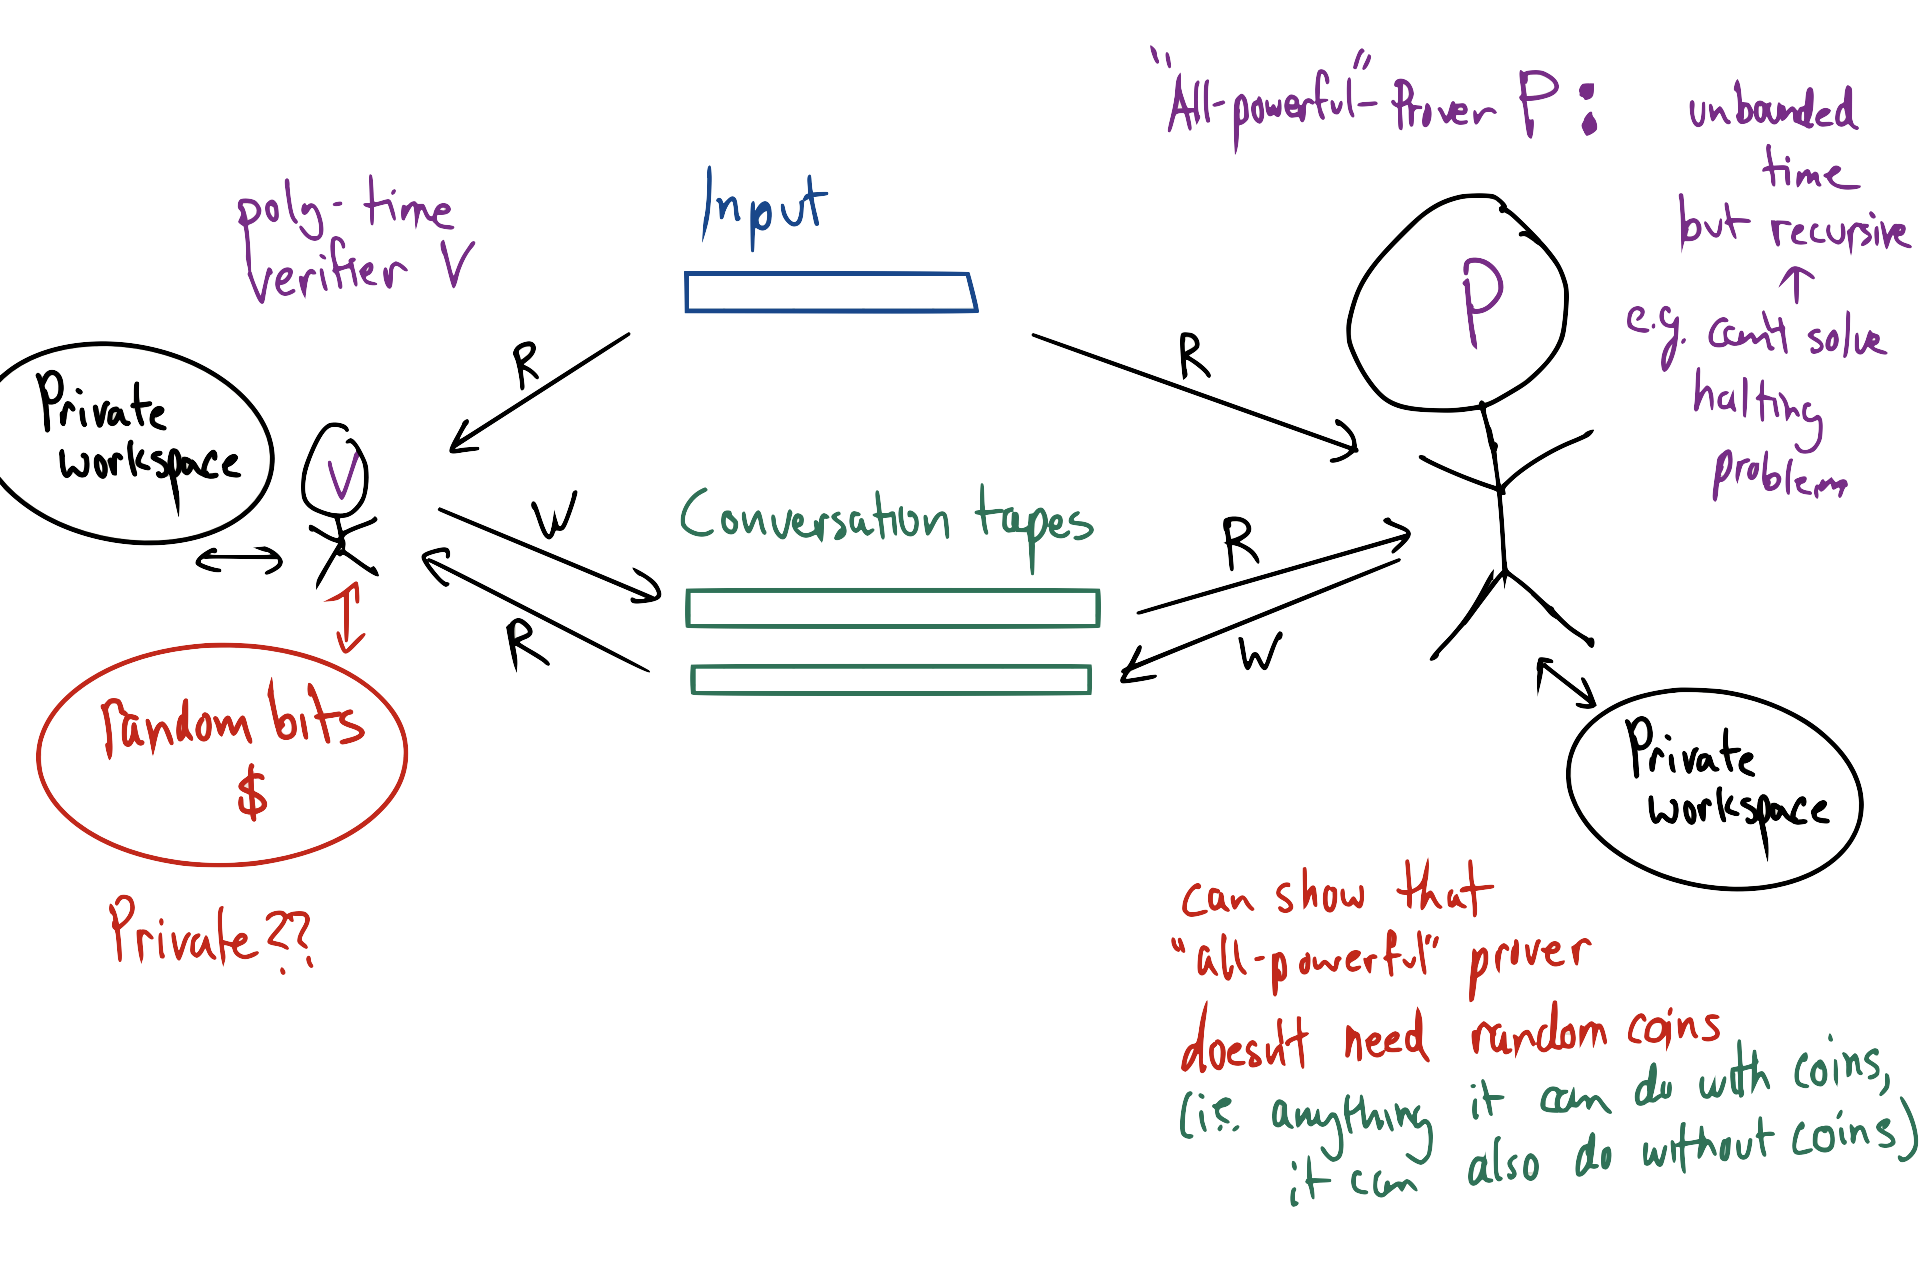
\includegraphics[width=\textwidth]{figures/ip.png}
  \caption{The model of interactive proofs.}
  \label{fig:ip}
\end{figure}

\begin{definition}[Goldwasser, Micali, Rackoff]
  An \emph{interactive proof system (IPS)} for a language $L$ is a protocol such that
  \begin{itemize}[itemsep=0pt]
    \item if $x \in L$ and both $V$ and $P$ follow the protocol, then $\PP_\text{coins of $V$}[\text{$V$ accepts $x$}] \geq 2/3$;
    \item if $x \not \in L$ and $V$ follows the protocol, then $\PP_\text{coins of $V$}[\text{$V$ rejects $x$}] \geq 2/3$.
  \end{itemize}
\end{definition}

\begin{definition}
  $\IP = \{ L \subset \{ 0, 1 \}^* : \text{$L$ has an IPS} \}$.
\end{definition}

By definition, $\NP \subseteq \IP$.

\begin{theorem}
  $\IP = \PSPACE$.
\end{theorem}

\begin{problem}[graph isomorphism, $\GI$]
  Given graphs $G$ and $H$, are they isomorphic?
\end{problem}

\begin{problem}[co-graph isomorphism, $\coGI$]
  Given graphs $G$ and $H$, are they not isomorphic?
\end{problem}

We know $\GI \in \NP$. It is unknown that $\coGI \in \NP$. However, $\coGI \in \IP$.

\begin{theorem}
  $\coGI \in \IP$.
\end{theorem}

\begin{proof}
  We give a protocol for $\coGI$, where $G_1$ and $G_2$ are graphs:
  \begin{enumerate}[label=(\roman*), itemsep=0pt]
    \item $V$ picks $c \in \{ 1, 2 \}$.
    \item $V$ picks a random labeling of vertices in $G_c$ and send the new adjacency matrix to $P$.
    \item $P$ guesses $c$.
    \item Repeat the above process for $k$ times.
  \end{enumerate}
  If $G_1 \not \cong G_2$, then $P$ can guess correctly every time. If $G_1 \cong G_2$, then $P$ needs to guess coin flips correctly each time, and $P$ can do this with probability at most $1/2^k$.
\end{proof}

Do $V$'s coins need to be private? In the example of $\coGI$, it \emph{seems} that if $P$ saw $V$'s choices, then it could cheat. However, Goldwasser and Sipser gives a surprising answer: anything that has a protocol with private coins also has a (possible different) protocol with public coins.

\begin{theorem}[Goldwasser, Sipser]
  $\IP_\text{private coins} = \IP_\text{public coins}$.
\end{theorem}

\end{document}
